\cotefile{91}
\scanpage{99}
\[
=\underset{\unsure{\mathfrak P|\mathcal P}}{\varinjlim}\;\underset{j}{\varprojlim}\;\deleted{\unsure{P|\alpha}}\prod_{\alpha}\operatorname{Hom}(X_{\alpha}^{\unsure{\mathfrak P|\mathcal P}},Y_j)
\]

\figure{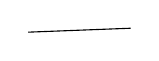
\begin{tikzpicture}\draw (0,0)--(1.3,.05);\end{tikzpicture}}

Ensembles quasi-\unsure{schématiques}.

\unsure{Les ens} \unsure{pro-schématiques} de type fini sur un
\deleted{\unsure{schéma}} \unsure{ens} \unsure{pro-schématique} \uline{\unsure{noethérien}}
\unsure{forment} une \uline{catégorie géométrique} (?)

\figure{\begin{tikzpicture}\draw (0,0)--(0,1);\end{tikzpicture}}
\margin{98}
\margin{\deleted{\unsure{4}}}
